\documentclass[10pt]{article}
\usepackage[margin=0.6in,top=0.5in,bottom=0.5in]{geometry}
\usepackage{amsmath,amssymb}
\usepackage{mathtools}
\usepackage[T1]{fontenc}
\usepackage{graphicx}
\usepackage{hyperref}

\pagestyle{empty}
\setlength{\parskip}{1pt plus 0.5pt}
\setlength{\abovedisplayskip}{4pt}
\setlength{\belowdisplayskip}{4pt}

\newcommand{\vW}{\mathbf{W}}
\newcommand{\vA}{\mathbf{A}}
\newcommand{\grad}{\nabla_{\!\vW}}

\begin{document}

\begin{center}
{\Large\bfseries Weight-space gradient descent induces approximate\\ activity descent, making learning rules testable}
\end{center}
\vspace{-2pt}
\begin{center}
\small
\href{https://github.com/koerding/ADescent}{GitHub} $\cdot$
\href{https://koerding.github.io/ADescent/}{Interactive Demo}
\end{center}
\vspace{-2pt}

\small

\paragraph{The problem: synaptic learning rules are hidden, but activity changes are not.}
A central question in neuroscience is whether biological neural networks optimise a loss function by adjusting synaptic weights---and if so, by what rule.  Decades of theoretical work have proposed candidate learning rules.  But synaptic weights cannot be measured at scale in behaving animals, so these proposals remain difficult to test directly.  Neural \emph{activities}, by contrast, can be recorded in large populations across learning.  This raises a concrete question: if the brain does perform gradient descent on its weights, what should we expect to see in the activities?  Here we show that the answer takes a surprisingly simple form---activity changes must be approximately proportional to activity-space loss gradients---and that this prediction is directly testable with existing experimental techniques.

\paragraph{Setup and derivation.}
Consider a feedforward network with layers $\ell=1,\ldots,L$, weights $\vW$, and neural activities $A_i^{(\ell)}(\vW)$, trained to minimise a loss $L$.  Gradient descent on the weights embodies a simple principle: \emph{the more that strengthening a synapse would improve performance, the more that synapse is strengthened} (and vice versa---harmful synapses are weakened).  Formally, every weight is updated simultaneously:
%
\begin{equation}
  \Delta W_\alpha = -\eta\,\frac{\partial L}{\partial W_\alpha}\,,
  \qquad \forall\;\alpha.
\end{equation}
%
What is the induced change in the activity of neuron $i$ in layer~$\ell$?
Because $A_i^{(\ell)}$ depends only on weights in layers $1$ through~$\ell$, the chain rule gives
%
\begin{equation}\label{eq:chain}
  \Delta A_i^{(\ell)}
  \;=\; -\eta \sum_{\alpha\in\text{layers}\,1..\ell} \frac{\partial A_i^{(\ell)}}{\partial W_\alpha}\,\frac{\partial L}{\partial W_\alpha}\,.
\end{equation}
%
In a feedforward network, the effect of any weight in layers $1..\ell$ on the loss passes entirely through the activities of layer~$\ell$, so $\partial L/\partial W_\alpha = \sum_{k\in\text{layer}\,\ell} (\partial L/\partial A_k^{(\ell)})\,(\partial A_k^{(\ell)}/\partial W_\alpha)$.  Exchanging the sums yields
%
\begin{equation}\label{eq:main}
  \boxed{\;\Delta A_i^{(\ell)} \;=\; -\eta \sum_{k\in\text{layer}\,\ell} \Phi^{(\ell)}_{ik}\;\frac{\partial L}{\partial A_k^{(\ell)}}\;,}
\end{equation}
%
where
%
\begin{equation}\label{eq:kernel}
  \Phi^{(\ell)}_{ik}
  \;\coloneqq\; \sum_\alpha \frac{\partial A_i^{(\ell)}}{\partial W_\alpha}\,\frac{\partial A_k^{(\ell)}}{\partial W_\alpha}
  \;=\; \grad A_i^{(\ell)} \cdot \grad A_k^{(\ell)}
\end{equation}
%
is a neural-tangent-kernel-style Gram matrix defined on the activities within each layer, and $\partial L/\partial A_k^{(\ell)}$ is the full backpropagated loss gradient---a sufficient statistic that compresses everything downstream layers contribute to the weight updates affecting layer~$\ell$.  In vector form, $\Delta\vA^{(\ell)} = -\eta\,\Phi^{(\ell)}\,\nabla_{\!\vA^{(\ell)}}L$: gradient descent in weight space induces \emph{kernel descent} within each layer of activity space.  This identity is exact and holds for any differentiable feedforward network, regardless of depth, width, or activation function.

\paragraph{The self term drives each neuron toward its own loss gradient.}
The diagonal element $\Phi^{(\ell)}_{ii}=\lVert\grad A_i^{(\ell)}\rVert^2$ collects contributions from \emph{all} weights that influence neuron $i$---both its own incoming weights and every weight in earlier layers that lies on a path to it.  Because $\Phi^{(\ell)}_{ii}>0$, the self term is always aligned with $-\partial L/\partial A_i^{(\ell)}$: each neuron's activity moves down its own loss gradient, with an effective learning rate $\eta\,\Phi^{(\ell)}_{ii}$ that grows with the depth and width of its input pathways.  In other words, weight-space gradient descent guarantees that every neuron has a built-in tendency to change its activity in the loss-reducing direction.

\paragraph{Cross terms introduce interference from other neurons.}
The off-diagonal elements $\Phi^{(\ell)}_{ik}=\grad A_i^{(\ell)}\cdot\grad A_k^{(\ell)}$ for $k\neq i$ couple neuron $i$ to every other neuron's loss gradient \emph{within the same layer}.  Their magnitude reflects parameter sharing: two neurons fed by overlapping early-layer weights will have large $|\Phi^{(\ell)}_{ik}|$; neurons in disjoint pathways will have $\Phi^{(\ell)}_{ik}\approx 0$.  These cross terms have no reason to be aligned with $-\partial L/\partial A_i^{(\ell)}$ and constitute interference---the side-effect of the rest of the layer learning simultaneously.  Whether the self term or the cross terms dominate determines whether activity changes look like activity-space gradient descent or something messier.

\paragraph{Wide networks make the kernel diagonal-dominant.}
The cross terms vanish when $\grad A_i^{(\ell)} \cdot \grad A_k^{(\ell)} \approx 0$ for $i\neq k$---that is, when different neurons' activities depend on nearly orthogonal directions in weight space.  Several settings push the kernel toward this regime.

\emph{Width.}  Two neurons in the same layer share no incoming weights, so their activity gradients are independent random vectors in parameter space.  By concentration of measure, their inner product scales as $O(1/\sqrt{d})$ while the diagonal scales as $O(1)$, making $\Phi^{(\ell)}$ increasingly diagonal-dominant as width grows---the internal-activity analogue of the NTK becoming deterministic at infinite width.

\emph{Depth and weight sharing.}  Neurons in the same layer share all earlier-layer weights, which introduces a common component into their parameter gradients.  Each neuron's own incoming weights act as independent random projections that decorrelate this shared component in the wide limit.  Deeper networks have more shared parameters but also more such projections; in practice, the cross terms remain significant at finite width.

\emph{Learning dynamics.}  Gradient descent itself may reinforce diagonal dominance.  Training is known to decorrelate neural representations as the network learns to tile the input space efficiently.  To the extent that decorrelated activities imply decorrelated parameter gradients---since $\partial A_i^{(\ell)}/\partial W_\alpha$ depends on upstream activations feeding into $i$---learning should progressively shrink the off-diagonal entries of $\Phi^{(\ell)}$.  The link between activity and gradient decorrelation is heuristic and deserves formal treatment, but it suggests that trained networks may be closer to the diagonal regime than their initializations.

Taken together, these arguments imply that in sufficiently wide networks---and cortical circuits are very wide---the kernel $\Phi^{(\ell)}$ is approximately diagonal, and activity changes closely track the negative activity-space loss gradient.

\paragraph{The diagonal approximation: activity descent as a proxy for weight descent.}
Combining the kernel identity (Eq.\,3) with diagonal dominance ($\Phi^{(\ell)}_{ii}\gg\sum_{k\neq i}|\Phi^{(\ell)}_{ik}|$) yields a simple approximation:
%
\begin{equation}\label{eq:diag}
  \Delta A_i^{(\ell)} \;\approx\; -\eta\,\Phi^{(\ell)}_{ii}\;\frac{\partial L}{\partial A_i^{(\ell)}}\,.
\end{equation}
%
The intuitive meaning mirrors that of weight descent: just as weight descent says \emph{strengthen each synapse in proportion to how much it helps}, activity descent says \emph{increase each neuron's firing in proportion to how much that increase would help} (and decrease it when it hurts).  Equation~5 shows that one implies the other in wide networks---the per-neuron scaling $\Phi^{(\ell)}_{ii}$ may differ across neurons, but every neuron's activity moves in the direction that locally reduces the loss.  This is the paper's central result: \emph{if a network performs gradient descent on its weights, and the network is wide enough, then its activity changes must approximately follow gradient descent in activity space.}  The approximation improves with width and, as our simulations show (Figs.\,1--2), is already accurate at moderate widths.

\paragraph{Recursive structure.}
The per-layer kernel inherits a recursion from the feedforward computation.  Writing $J_\ell = \partial\vA^{(\ell)}/\partial\vA^{(\ell-1)}$ for the inter-layer Jacobian and $D_\ell = \mathrm{diag}([\sigma'(z_i^{(\ell)})]^2\,\lVert\vA^{(\ell-1)}\rVert^2)$ for the diagonal kernel from layer~$\ell$'s own incoming weights:
%
\begin{equation}\label{eq:phi-recursion}
  \Phi^{(\ell)} = D_\ell + J_\ell\,\Phi^{(\ell-1)}\,J_\ell^T\,,
  \qquad
  \Phi^{(1)} = D_1\,.
\end{equation}
%
$D_\ell$ is always diagonal---own-layer weights never couple same-layer neurons.  All off-diagonal structure comes from $J_\ell\,\Phi^{(\ell-1)}\,J_\ell^T$: earlier-layer weight updates propagated forward.  Width decorrelates $J_\ell$ at every stage, so diagonal dominance strengthens recursively.

\paragraph{A testable prediction for neuroscience.}
This result converts an untestable claim about synaptic learning rules into a testable prediction about observable activity changes.  Synaptic weights cannot be measured at scale in vivo, but neural activities can.  If a biological circuit performs \emph{any} form of gradient descent on its synaptic weights---even an approximate or noisy variant---and is sufficiently wide that $\Phi^{(\ell)}$ is diagonal-dominant, then the observable activity changes must satisfy Eq.\,5.  The per-neuron scaling $\Phi^{(\ell)}_{ii}$ is unknown and may vary across neurons, but the \emph{direction} of $\Delta\vA^{(\ell)}$ is pinned: it must be approximately proportional to $-\nabla_{\!\vA^{(\ell)}}L$.  A concrete experimental protocol follows: record neural population activity across learning trials, estimate $\partial L/\partial A_i^{(\ell)}$ from a task-fitted model, and check whether the measured $\Delta A_i^{(\ell)}$ is proportional to the predicted gradient.  Only the direction matters, not the magnitude---the unknown $\Phi^{(\ell)}_{ii}$ absorbs all per-neuron scaling.  A failure of proportionality would rule out not just backpropagation but \emph{any} weight-space gradient rule in a network wide enough for diagonal dominance.

\paragraph{Caveat: activity descent is necessary but not sufficient for weight descent.}
The converse is weaker: observing that activities follow their loss gradient constrains the projection of $\Delta\vW$ onto the row space of the Jacobian $\partial A_i^{(\ell)}/\partial W_\alpha$, but says nothing about the (typically vast) null space of weight changes that leave activities unchanged on the current input.  Activity-level gradient descent is therefore consistent with many different weight-level learning rules, of which backpropagation is the minimum-norm solution.  In short, weight descent implies activity descent (in wide networks), but activity descent does not uniquely identify the weight-level rule.  This asymmetry is a feature, not a bug: it means the test can \emph{falsify} gradient-based learning, even though it cannot confirm a specific synaptic rule.

\paragraph{Methods.}
Figures~1--2 numerically verify Eqs.\,2--5 in a 3-hidden-layer ReLU MLP trained with online SGD ($\eta=0.005$) on a 2-class image dataset (4$\times$4 pixel images of horizontal vs.\ vertical bars, 20 per class, input dimension 16, output dimension 2).  Dead ReLU neurons (pre-activation $\leq 0$ on the sampled input) are excluded from all analyses.  At regular intervals during training, we compute the full activity Jacobian $\partial A_i^{(\ell)}/\partial W_\alpha$ and the per-layer kernel $\Phi^{(\ell)}_{ik}$, then compare the predicted activity change $\Delta A$ from the chain-rule identity (Eq.\,2), the kernel equation (Eq.\,3), and the diagonal approximation (Eq.\,5) against the actual change measured after a single gradient step.  Figure~1 shows detailed diagnostics at widths 8 and 48.  Figure~2 sweeps width from 4 to 128 (3 random seeds per width, each trained for 2000 SGD steps) to quantify how the diagonal approximation improves with width.

\newpage
\begin{figure}[h!]
\centering
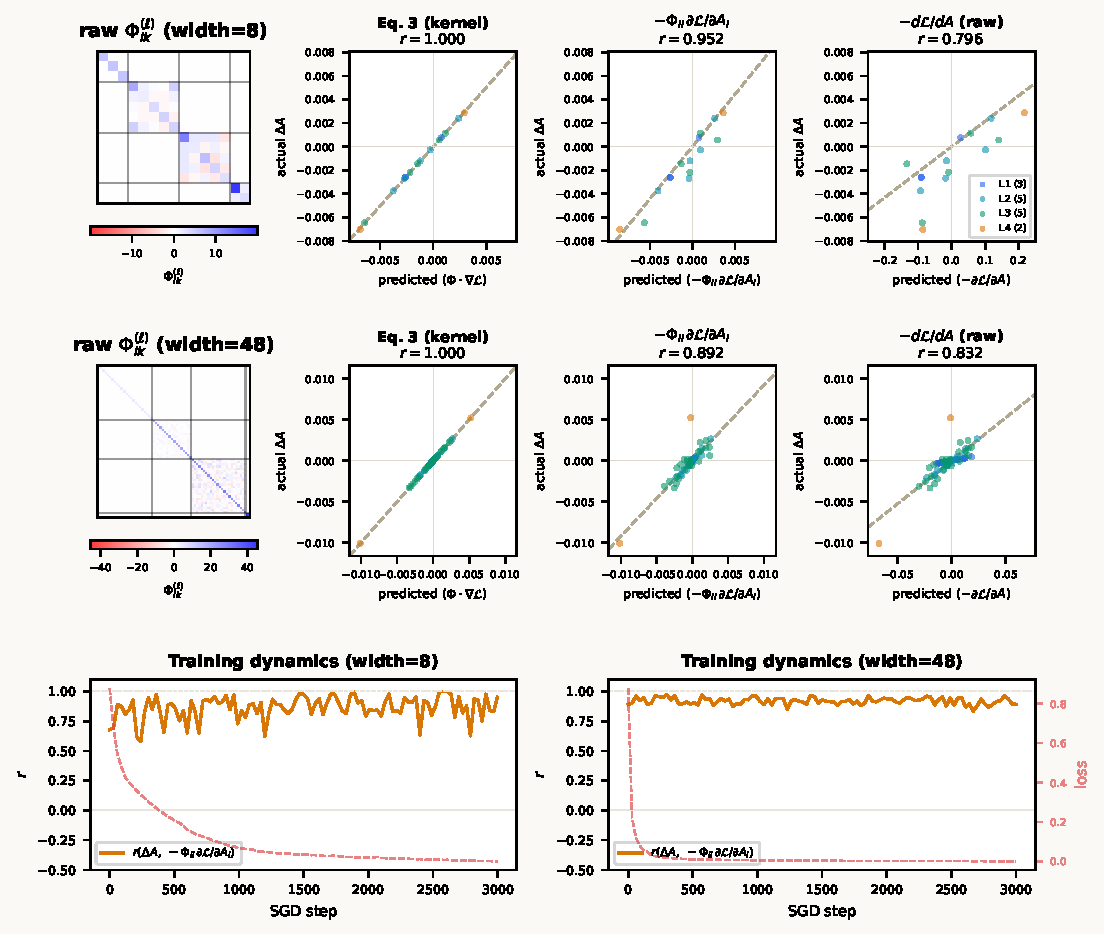
\includegraphics[width=\textwidth]{fig_ntk.pdf}
\caption{\textbf{In a wide network doing weight descent, activity changes closely match activity-space gradient descent.}  Top row: width\,=\,8.  Middle row: width\,=\,48.  Left: normalised $\Phi^{(\ell)}_{ik}$ heatmaps (white = uncorrelated, blue = correlated).  Scatter panels: predicted vs.\ actual $\Delta A$ for the full kernel (Eq.\,3), the diagonal approximation (Eq.\,5), and raw $-\partial L/\partial A$.  Dead ReLU neurons excluded.  Bottom row: $r(\Delta A,\,-\partial L/\partial A)$ and loss over training.}
\end{figure}

\begin{figure}[h!]
\centering
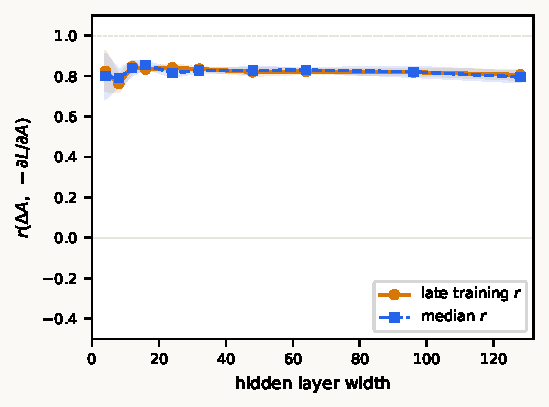
\includegraphics[width=0.55\textwidth]{fig_width_sweep.pdf}
\caption{\textbf{The wider the network, the more faithfully activity changes track the activity-space loss gradient.}  Pearson $r$ between actual $\Delta A$ and $-\partial L/\partial A$ as a function of hidden-layer width.  Dead ReLU neurons excluded.  Shaded regions: $\pm1$ s.d.\ across seeds.}
\end{figure}

\newpage
\appendix

\section*{Appendix A. He initialisation, depth, and the $\sqrt{3}/2$ baseline}

This appendix asks how the correlation $r(\Delta\vA,\,-\nabla_{\!\vA}L)$ depends on depth $D$ under He (Kaiming) initialisation, $W^{(\ell)}_{ij}\sim\mathcal{N}(0,\,2/n_{\ell-1})$ (\texttt{gen\_figures.py}, line~20).  A leading-order calculation predicts an explicit number; empirically the prediction is matched at small depth but breaks down as $D$ grows.  Both pieces of information are useful.

\paragraph{Three variance-preservation properties of He init.}
For a ReLU MLP at initialisation, in the wide-Gaussian limit:
\begin{enumerate}
\setlength\itemsep{0pt}
  \item[(i)] \emph{Forward signal preserved}: $\mathbb{E}\lVert\vA^{(\ell)}\rVert^2/n_\ell$ is independent of $\ell$ (design property of He init for ReLU).
  \item[(ii)] \emph{Backward signal preserved}: $\mathbb{E}\lVert\partial L/\partial\vA^{(\ell)}\rVert^2/n_\ell$ is also independent of $\ell$, by the dual He calculation.
  \item[(iii)] \emph{Per-layer Jacobian norms preserved}: $\mathbb{E}\lVert J^{(\ell\leftarrow m)}_{i,:}\rVert^2 = O(1)$, independent of $\ell-m$.
\end{enumerate}

\paragraph{A leading-order calculation predicts $\sqrt{3}/2$.}
Decompose
\begin{equation}\label{eq:phi-ii-sum}
  \Phi^{(\ell)}_{ii}\;=\;\sum_{m=1}^{\ell}\bigl(\sigma'_i\bigr)^2\,\lVert J^{(\ell\leftarrow m+1)}_{i,:}\rVert^2\,\lVert\vA^{(m-1)}\rVert^2.
\end{equation}
By (i) and (iii) each summand has the same distribution, with mean of order $n$, so to leading order $\Phi^{(\ell)}_{ii}\approx\ell\cdot\kappa\cdot n$ for a He-determined constant $\kappa$.  Treating $\sigma'_i$, $g_i\coloneqq\partial L/\partial A^{(\ell)}_i$, and the realisation of $\lVert J\rVert^2$ as i.i.d.\ across $(\ell,i)$, and $\ell$ as approximately uniform on $\{1,\dots,D\}$:
\begin{equation}\label{eq:r-derivation}
  r\bigl(\Delta\vA,\,-\nabla_{\!\vA}L\bigr)
  \;\approx\;\frac{\mathbb{E}[\ell]}{\sqrt{\mathbb{E}[\ell^2]}}
  \;\xrightarrow{D\to\infty}\;\frac{\sqrt{3}}{2}\;\approx\;0.866.
\end{equation}
The $D$'s cancel: the limiting value is set by the \emph{shape} of $\Phi^{(\ell)}_{ii}\propto\ell$, which itself is forced by He's variance-preservation property.

\begin{figure}[h!]
\centering
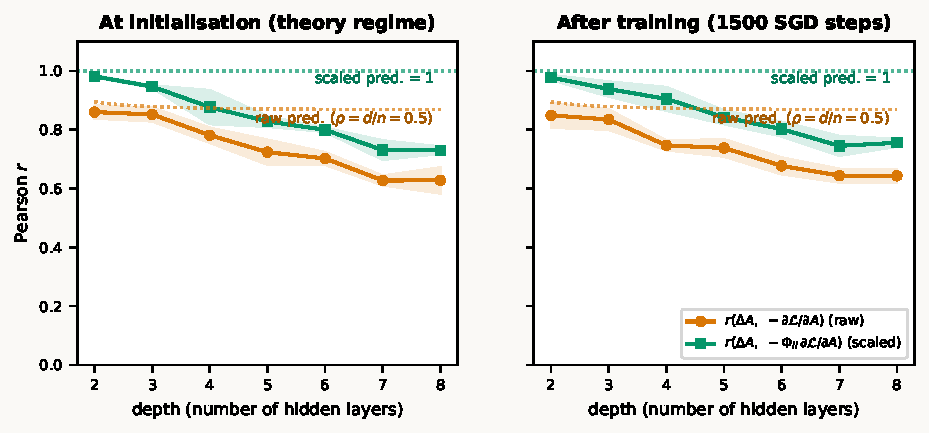
\includegraphics[width=0.95\textwidth]{fig_depth_sweep.pdf}
\caption{\textbf{Depth sweep at fixed width ($n=32$, 3 seeds).}  Pearson $r$ between actual $\Delta\vA$ and the gradient signal, plotted against network depth.  Orange: raw gradient $-\partial L/\partial A$.  Green: gradient scaled by $\Phi^{(\ell)}_{ii}$.  Left panel averages the first 3 diagnostics (initialisation regime); right panel averages the last 5 diagnostics (after 1500 SGD steps).  Dotted line marks the leading-order prediction $\sqrt{3}/2$ from Eq.\,\ref{eq:r-derivation}.}\label{fig:depth-sweep}
\end{figure}

\paragraph{Where the prediction holds and where it breaks.}
Fig.\,\ref{fig:depth-sweep} sweeps depth from 2 to 8 at fixed width $n=32$ and reports the raw and scaled correlations both at initialisation and after training.  Three things are visible:
\begin{enumerate}
\setlength\itemsep{0pt}
  \item \emph{The $\sqrt{3}/2$ baseline lands.}  At depth 2 the raw correlation is $\approx 0.86$, essentially the predicted value $\sqrt{3}/2\approx 0.866$.  The shape of the calculation is right.
  \item \emph{Init and trained behave nearly identically.}  The left and right panels are within noise of each other, so the depth-dependence is a property of the initialisation regime itself, not a consequence of training.
  \item \emph{Both correlations decrease with depth.}  At $D=8$, raw $r$ drops to $\approx 0.63$ and scaled $r$ to $\approx 0.73$.  The leading-order calculation predicts flatness for the raw correlation and an approach to $1$ for the scaled correlation; the data contradict both.
\end{enumerate}
The decrease has two probable sources, both invisible to the leading-order argument.  First, the calculation treats $\Phi^{(\ell)}_{ii}$ as deterministically equal to $\ell\kappa n$ within a layer; at finite width $n=32$ the within-layer scatter of $\Phi^{(\ell)}_{ii}$ is non-negligible, contributing noise that compounds across $D$ pooled layers.  Second, the layer-wise gradients $\partial L/\partial\vA^{(\ell)}$ are not i.i.d.\ across $\ell$: backprop produces them as $\bigl(J^{(L\leftarrow\ell+1)}\bigr)^{\!\top}\!(\vA^{(L)}-\vy)$, so they share the output error and inherit cross-layer correlation that grows with depth.  Both effects are $O(1/n)$ per layer and accumulate over $D$ layers.

\paragraph{Implication.}
The appropriate reading is that $\sqrt{3}/2$ is a wide-network, shallow-depth approximation set by the variance-preservation property of He init.  At width $n=32$ it is accurate for $D\le 3$; for larger $D$ the correlation falls because the i.i.d.\ assumptions in Eq.\,\ref{eq:r-derivation} fail.  The interactive demo allows the reader to verify both panels of Fig.\,\ref{fig:depth-sweep} live.

\end{document}
